\appendix
\section{Selection}
\begin{table}[H]
    \centering
    \begin{enumerate}
    \item Integrated Charge $>$ 0.6 pC
    \item Sum Trigger Waveform Peaktime $\in$ (-0.7 $\mu s$,-0.5 $\mu s$)
    \item Average Charge In Background Channels $<$ 0.2 pC
    \end{enumerate}
    \caption{Integrated Charge Based Selection Criteria}
    \label{tab:my_label}
\end{table}

\begin{table}[H]
    \centering
    \begin{enumerate}
    \item Pulse Height $>$ 50 mV
    \item Sum Trigger Waveform Peaktime $\in$ (-0.7 $\mu s$,-0.5 $\mu s$)
    \item Average Charge In Background Channels $<$ 0.2 pC
    \end{enumerate}
    \caption{Pulse Amplitude Based Selection Criteria}
    \label{tab:my_label}
\end{table}
All charge values are gain corrected by direct measurement or by measured mean of production lot if direct measurement isn't possible.

\subsection{Integrated Charge vs. Pulse Amplitude}
Here we have compared the impact of placing a threshold on two alternate attributes of the individual MPPC signal waveforms -- maximum pulse height and integrated charge under the waveform pulse. We used a fit of the interpolated FARO grid for all 4092 MPPC positions (uncertainties on these positions are much less than required for our 1 mm bin size) in order to combine scan data from all Z-Scanned MPPCs. Shown in , we find that while there is the expected, high correlation between amplitude and charge, the width of this uncertainty is perhaps larger that was anticipated. Therefore, despite the values of our two cuts being roughly equivalent on average, the width of this distribution still allows for significant differences in event selection.

\begin{figure}
    \centering
    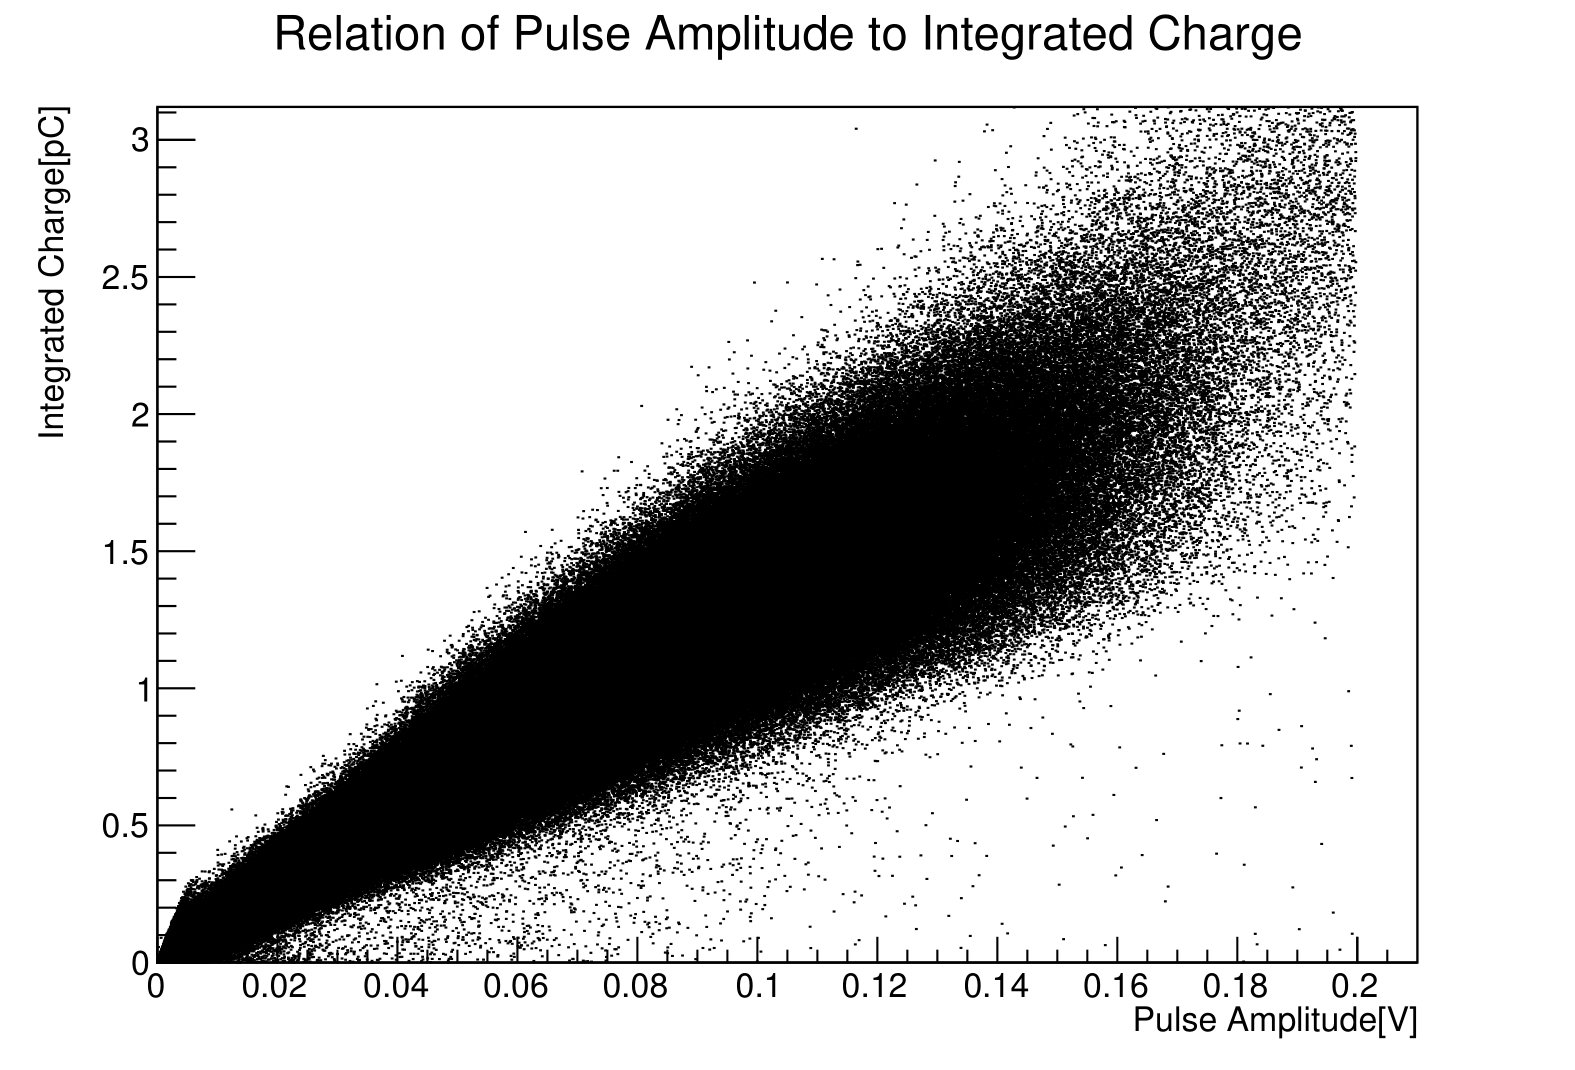
\includegraphics[width=5cm]{graphics/qvamp-1.png}
    \caption{Relationship of height to charge in a single event waveform}
    \label{fig:qvsamp}
\end{figure}

Particularly of note is that there are significant differences in this relation across the face of individual MPPCs.
Figure \ref{fig:heightvzplot} shows this via the net average mppc charge and height behaviour v. position across all scanned mppcs.
From a polynomial fit of both of these figures, we find, as agrees with prior findings, that the peaks of the charge measurements agree with our previous results of a 10\% drop in the downboard half. For height, the same effect still appears but to a much lesser extent.

\begin{figure}
\centering

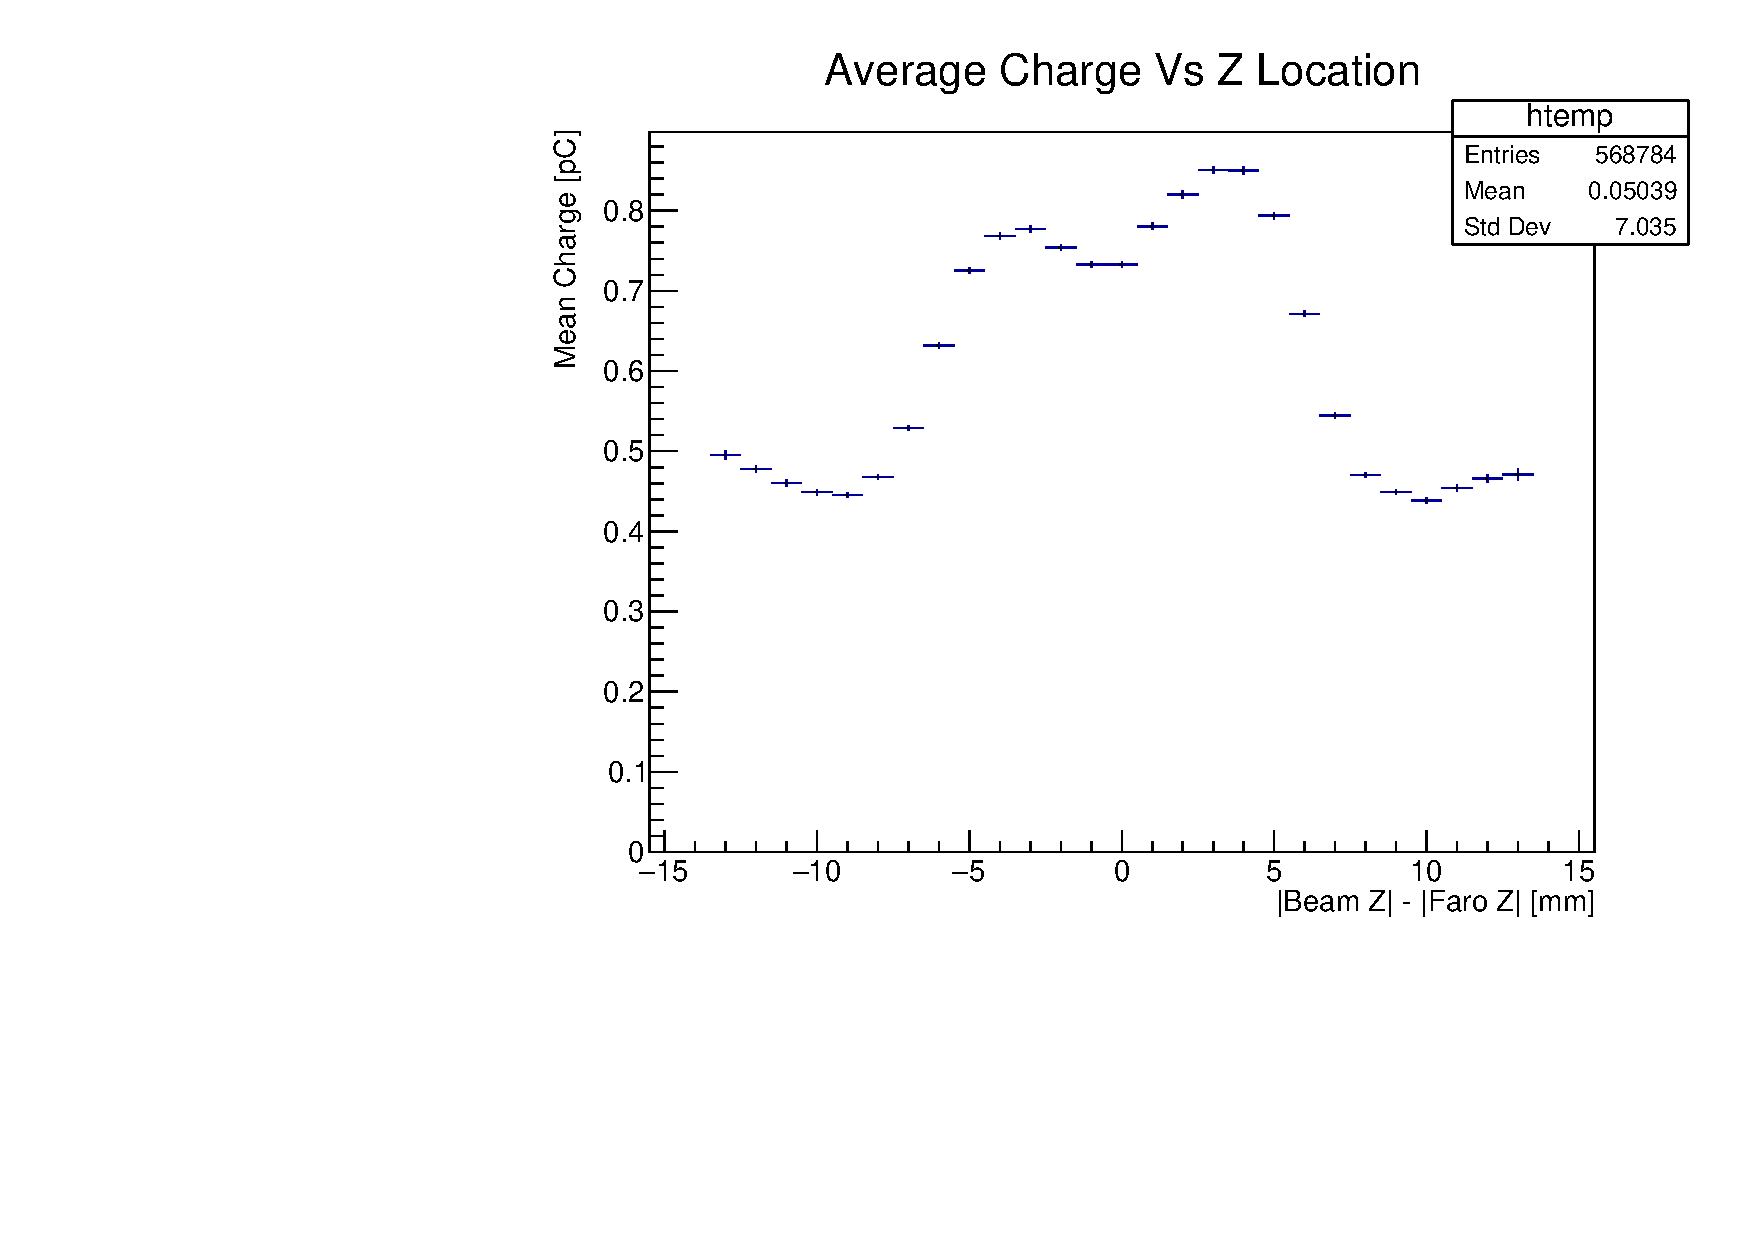
\includegraphics[width=4 cm]{graphics/chargevsz.pdf}
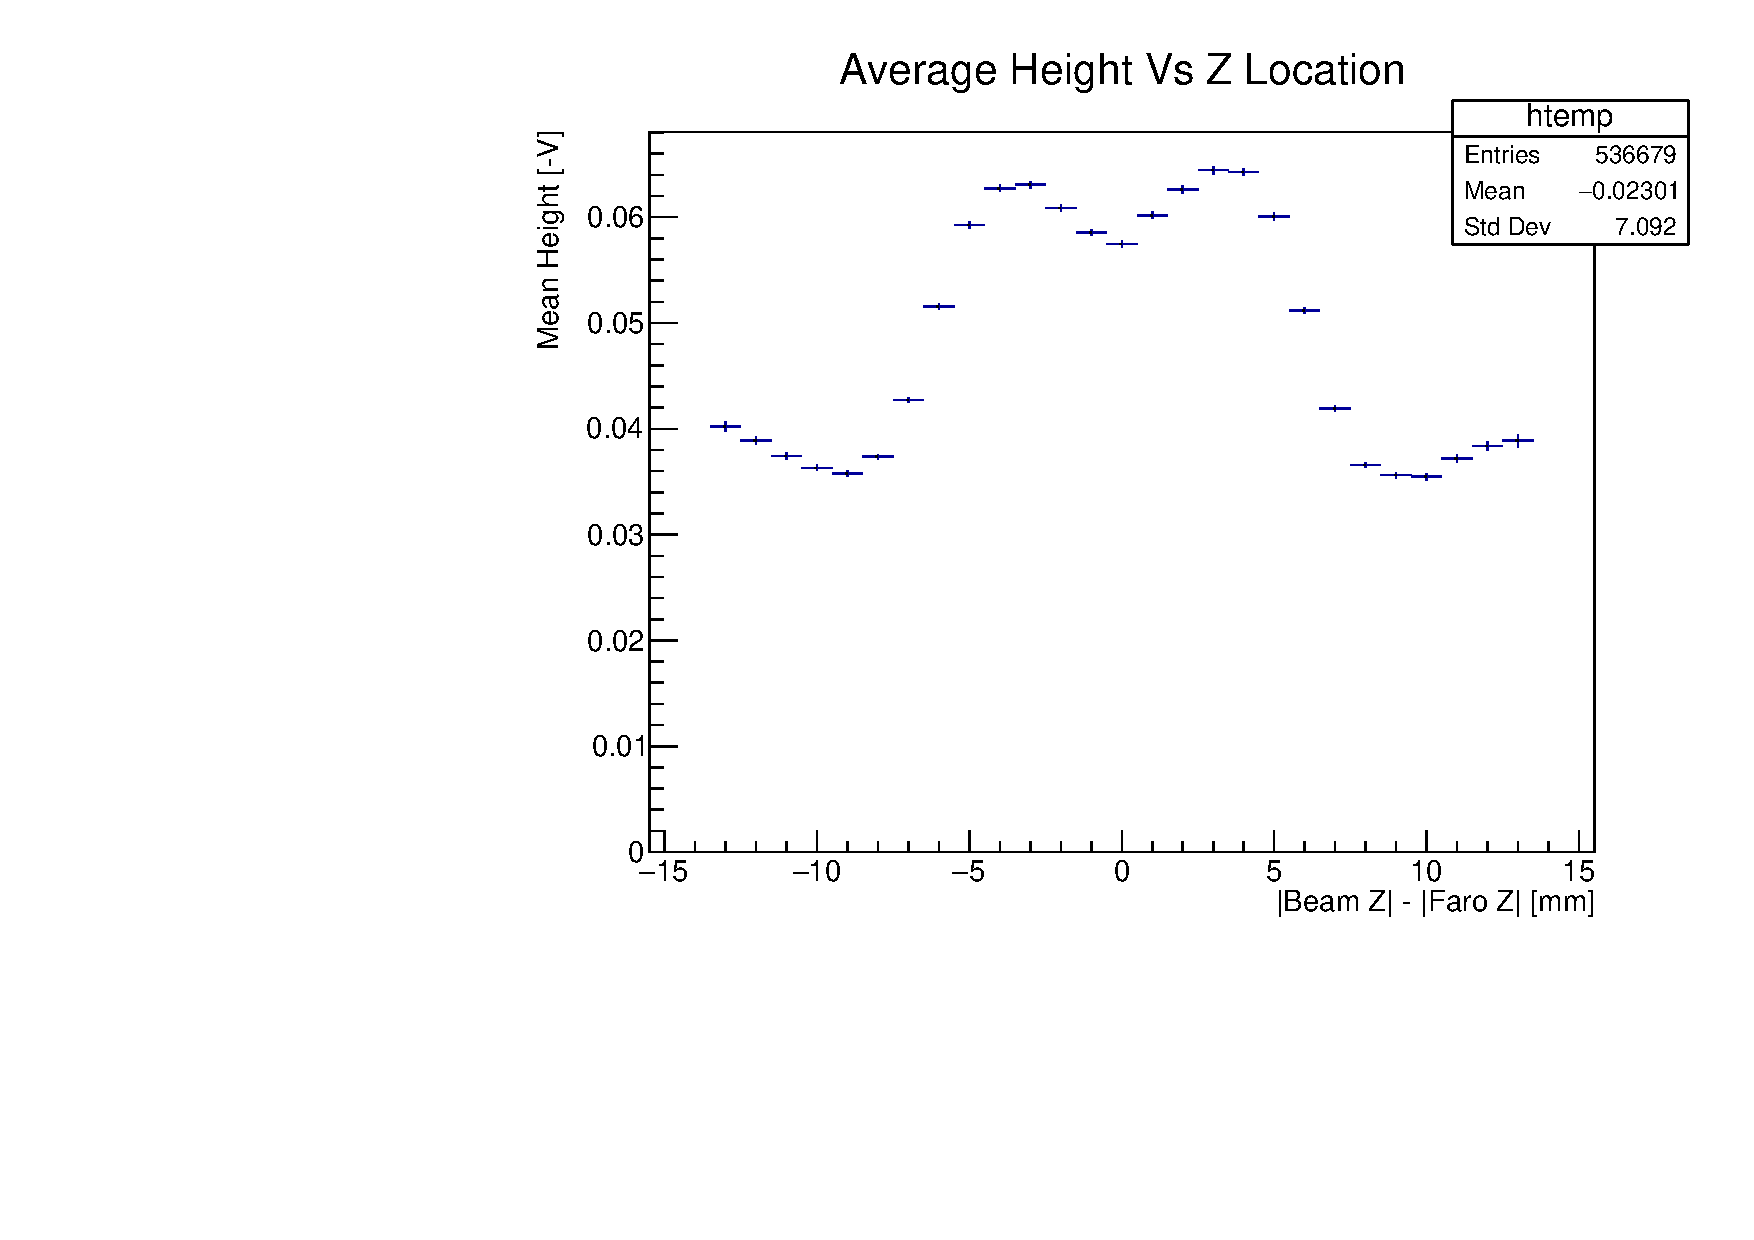
\includegraphics[width=4 cm]{graphics/heightvsz.pdf}
\caption{Average charge (left), height (right) in an event relative to measurement location on MPPC}
\label{fig:heightvzplot}
\end{figure}

\begin{figure}
\centering
    
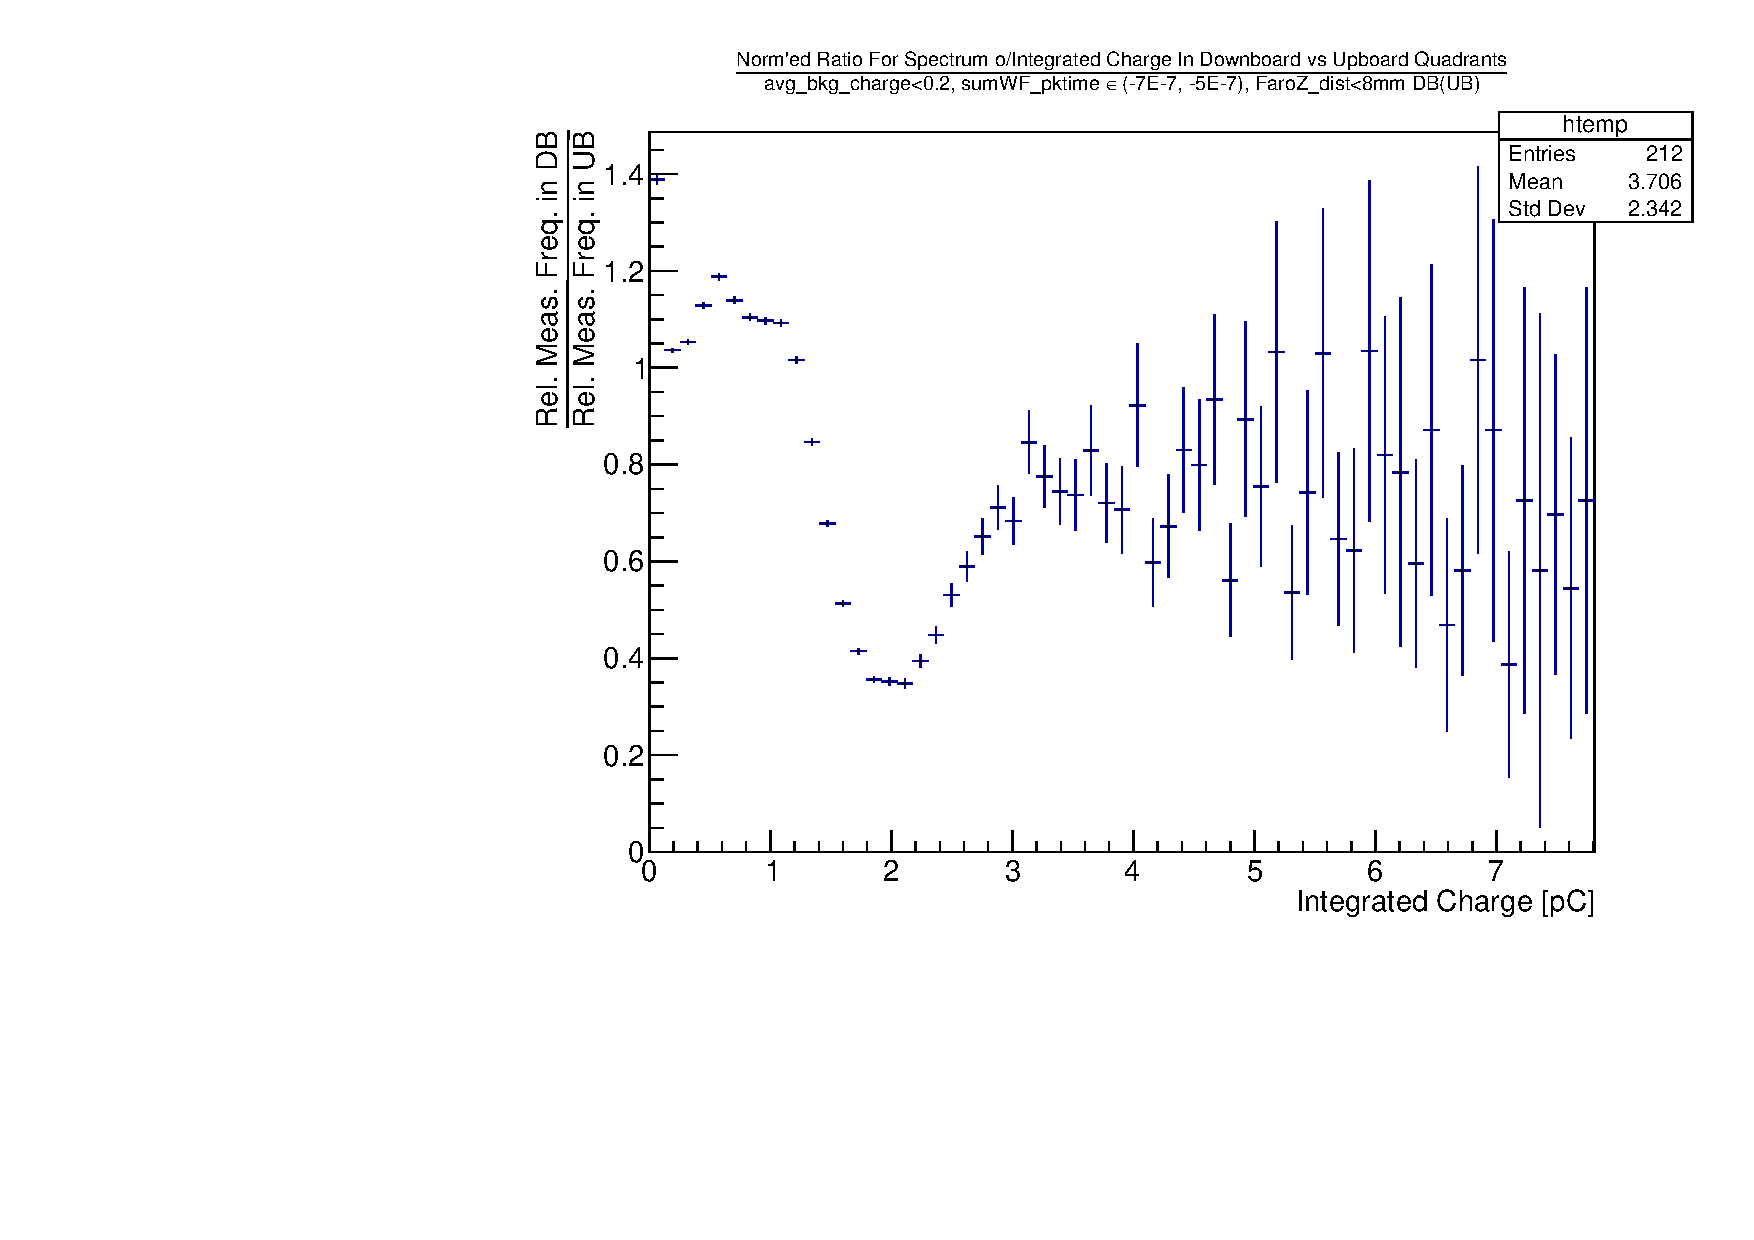
\includegraphics[width=4 cm]{graphics/chargeratiospectrum_DBtoUB.pdf}
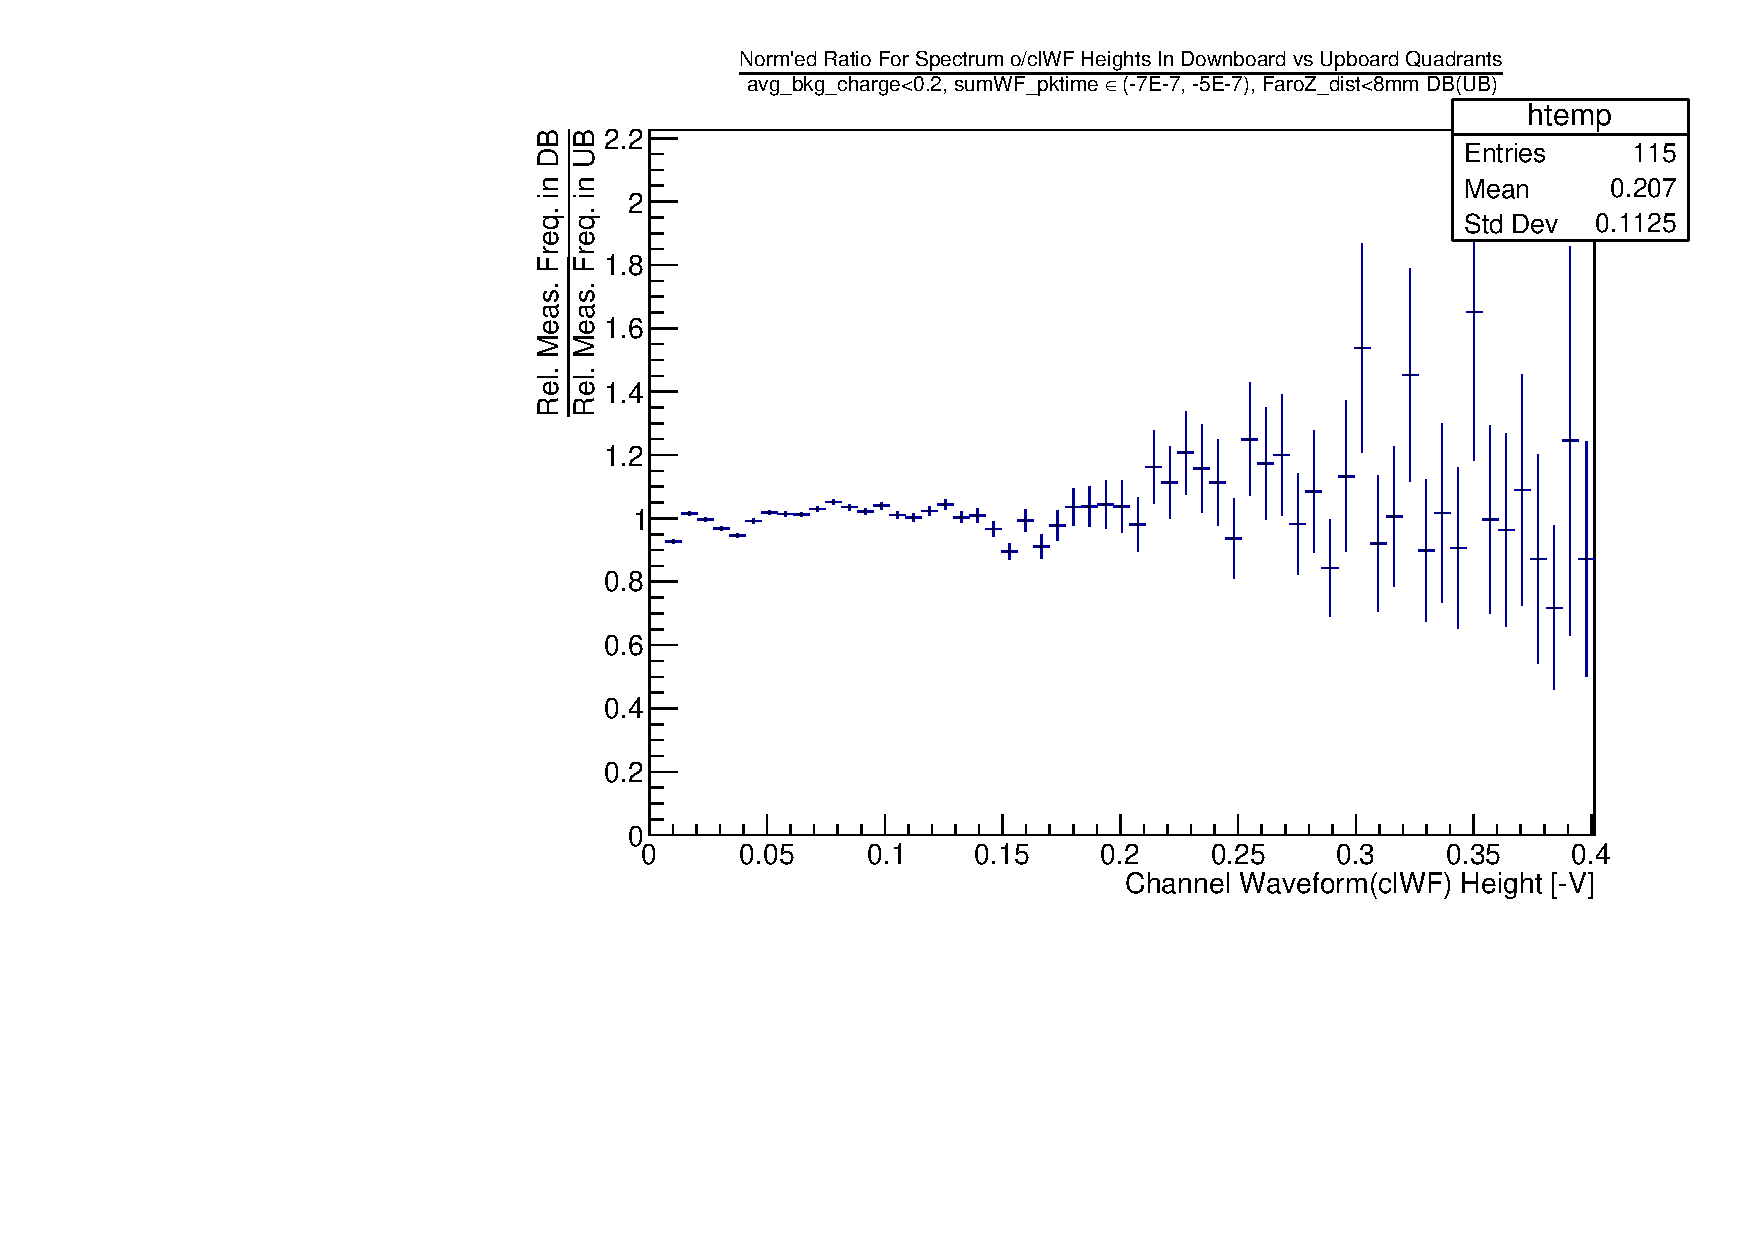
\includegraphics[width=4 cm]{graphics/heightratiospectrum_DBtoUB.pdf}
\caption{Ratio of normalized charge (left), height (right) distributions in each MPPC half}
\label{fig:heightspectrumplot}
\end{figure}

\begin{table}[H]
    \centering
    \begin{tabular}{c||c|c|c}
         & DB Peak & UB Peak & Ratio \\
         \hline
        Charge & 0.777548 pC & 0.860434 pC & 0.903669 \\
        Height & 63.336 mV & 65.0873 mV & 0.973094
    \end{tabular}
    \caption{Amplitude of Height and Charge Distributions For MPPC Halves }
    \label{tab:qandhhalves}
\end{table}




Additionally, we are interested in the relative response between the two MPPC halves across the range of charge and height measurements.
Figure \ref{fig:heightspectrumplot} is especially interesting because these plots allow us to determine the differential nature in which the two sides will be effected by any alterations to the chosen threshold value. In the region of our selection criteria, the charge threshold will reject a higher number of events on the side closer to Z=0, whereas a selection on height effect both sides of the mppc equally. Moreover, this shift is in fact confirmed when we analyze the found mppc positions from both cuts, where a clear shift outwards from zero is present in the charge based cuts (Fig. \ref{fig:seldzvz}).
\begin{figure}
    \centering
    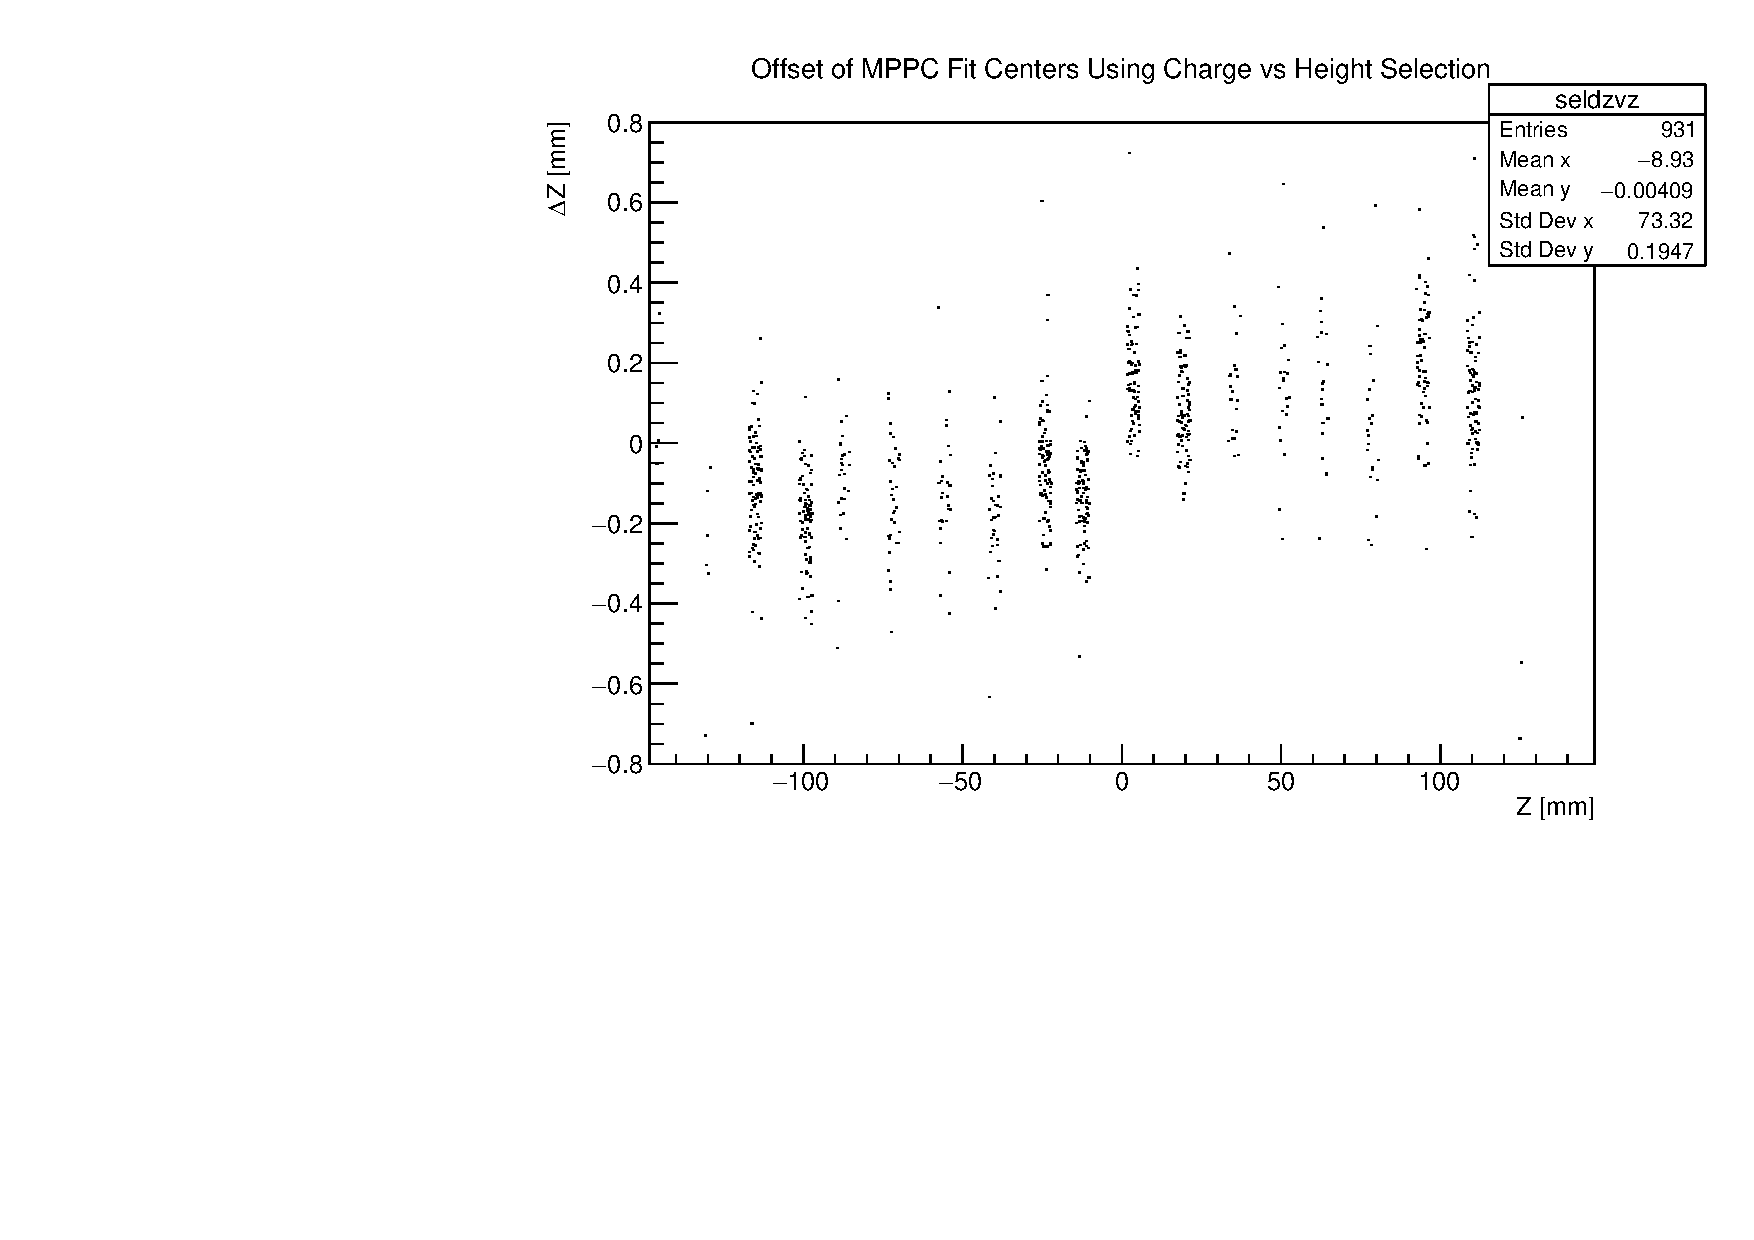
\includegraphics[width=5cm]{graphics/selectionshiftoverz.pdf}
    \caption{Difference in found positions under change from charge to amplitude selection}
    \label{fig:seldzvz}
\end{figure}








\section{Alternate Fit Function}
The set of well fit MPPCs were selected using the following critia,
\begin{enumerate}
    \item Uncertainty In Fit Mean $<$ 0.5 mm
    \item Uncertainty In Fit Sigma $<$ 0.5 mm
    \item Fit Width $\in$ (5.5mm,8.5mm)
    \item Reduced $\chi ^{2} \; <$ 4
\end{enumerate}

Comparing this set to the found positions from the piecewise fit function, we find the distribution contains very small offsets

\begin{figure}[h]
    \centering
    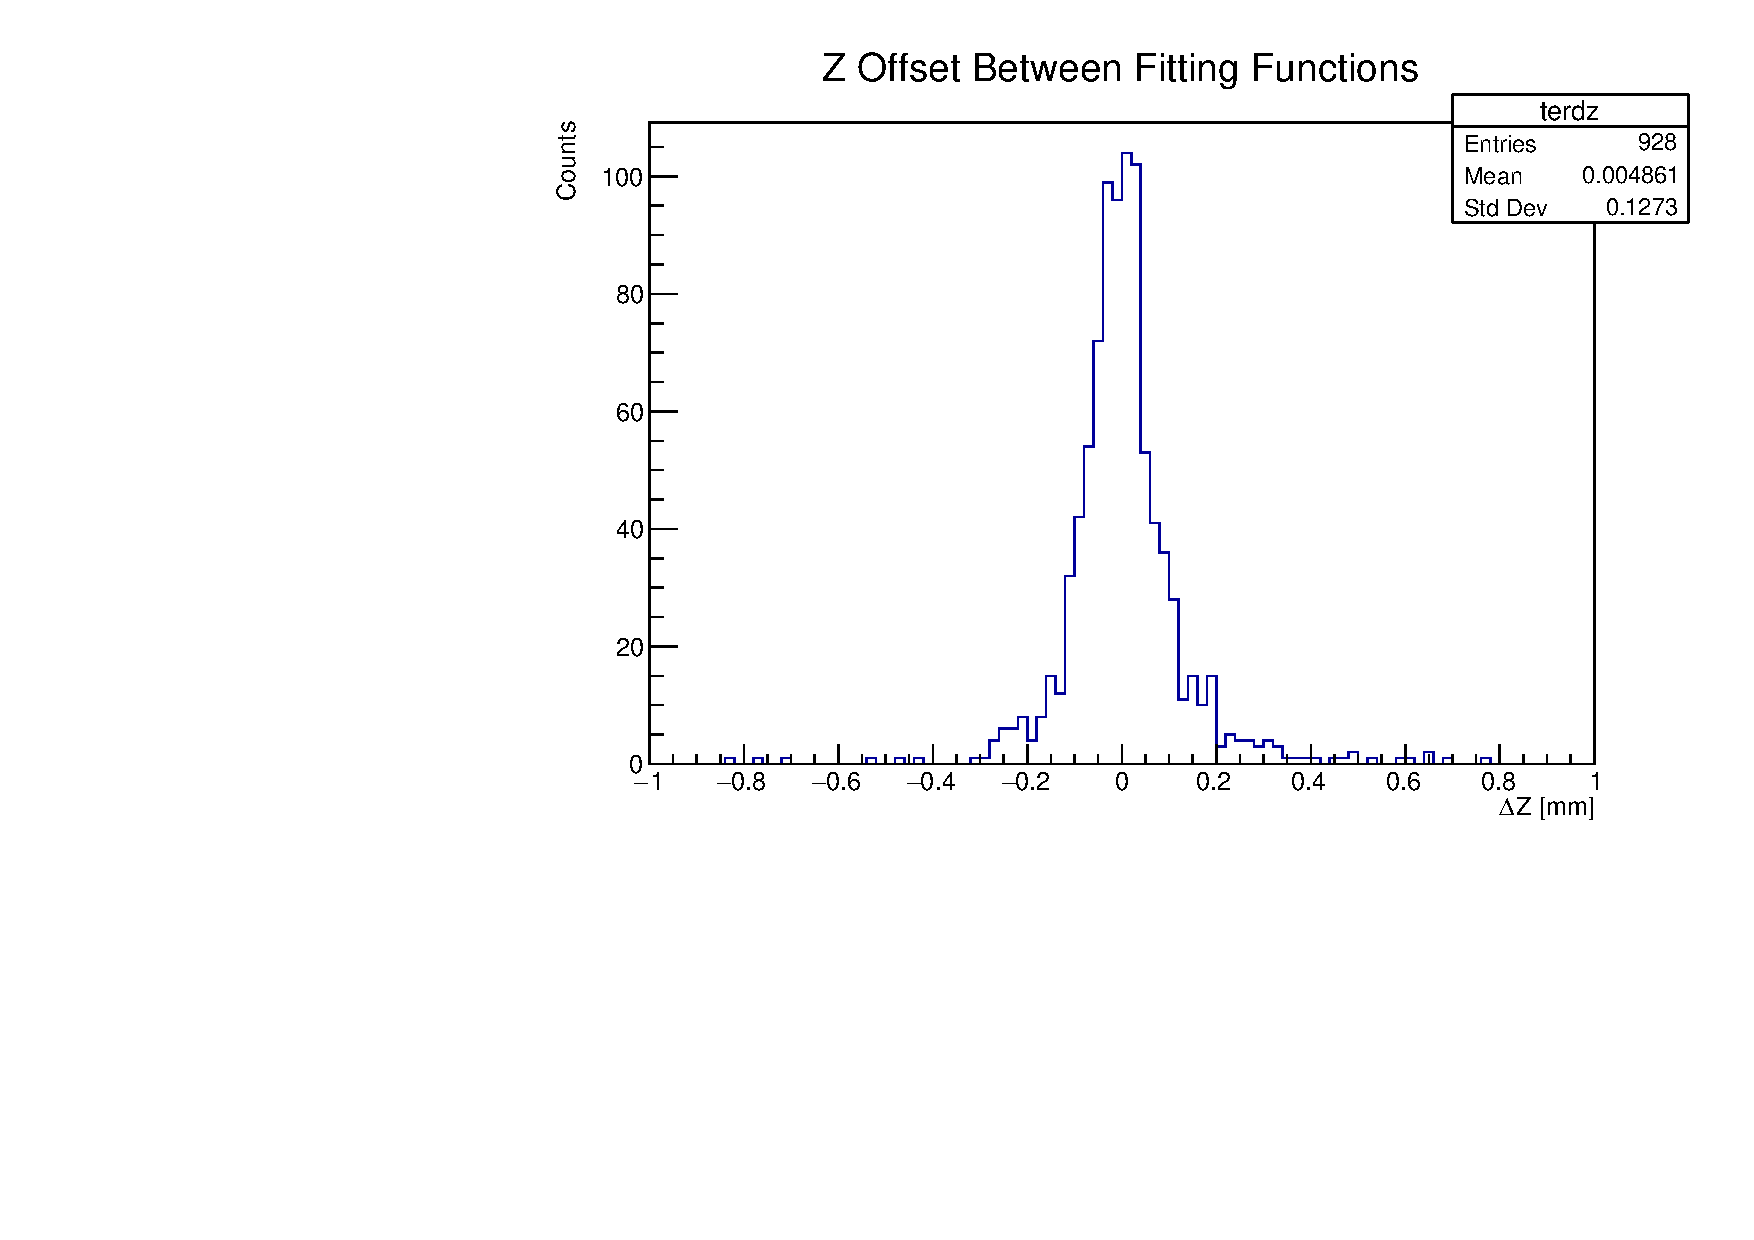
\includegraphics[width=.7\linewidth]{graphics/terdzhc.pdf}
    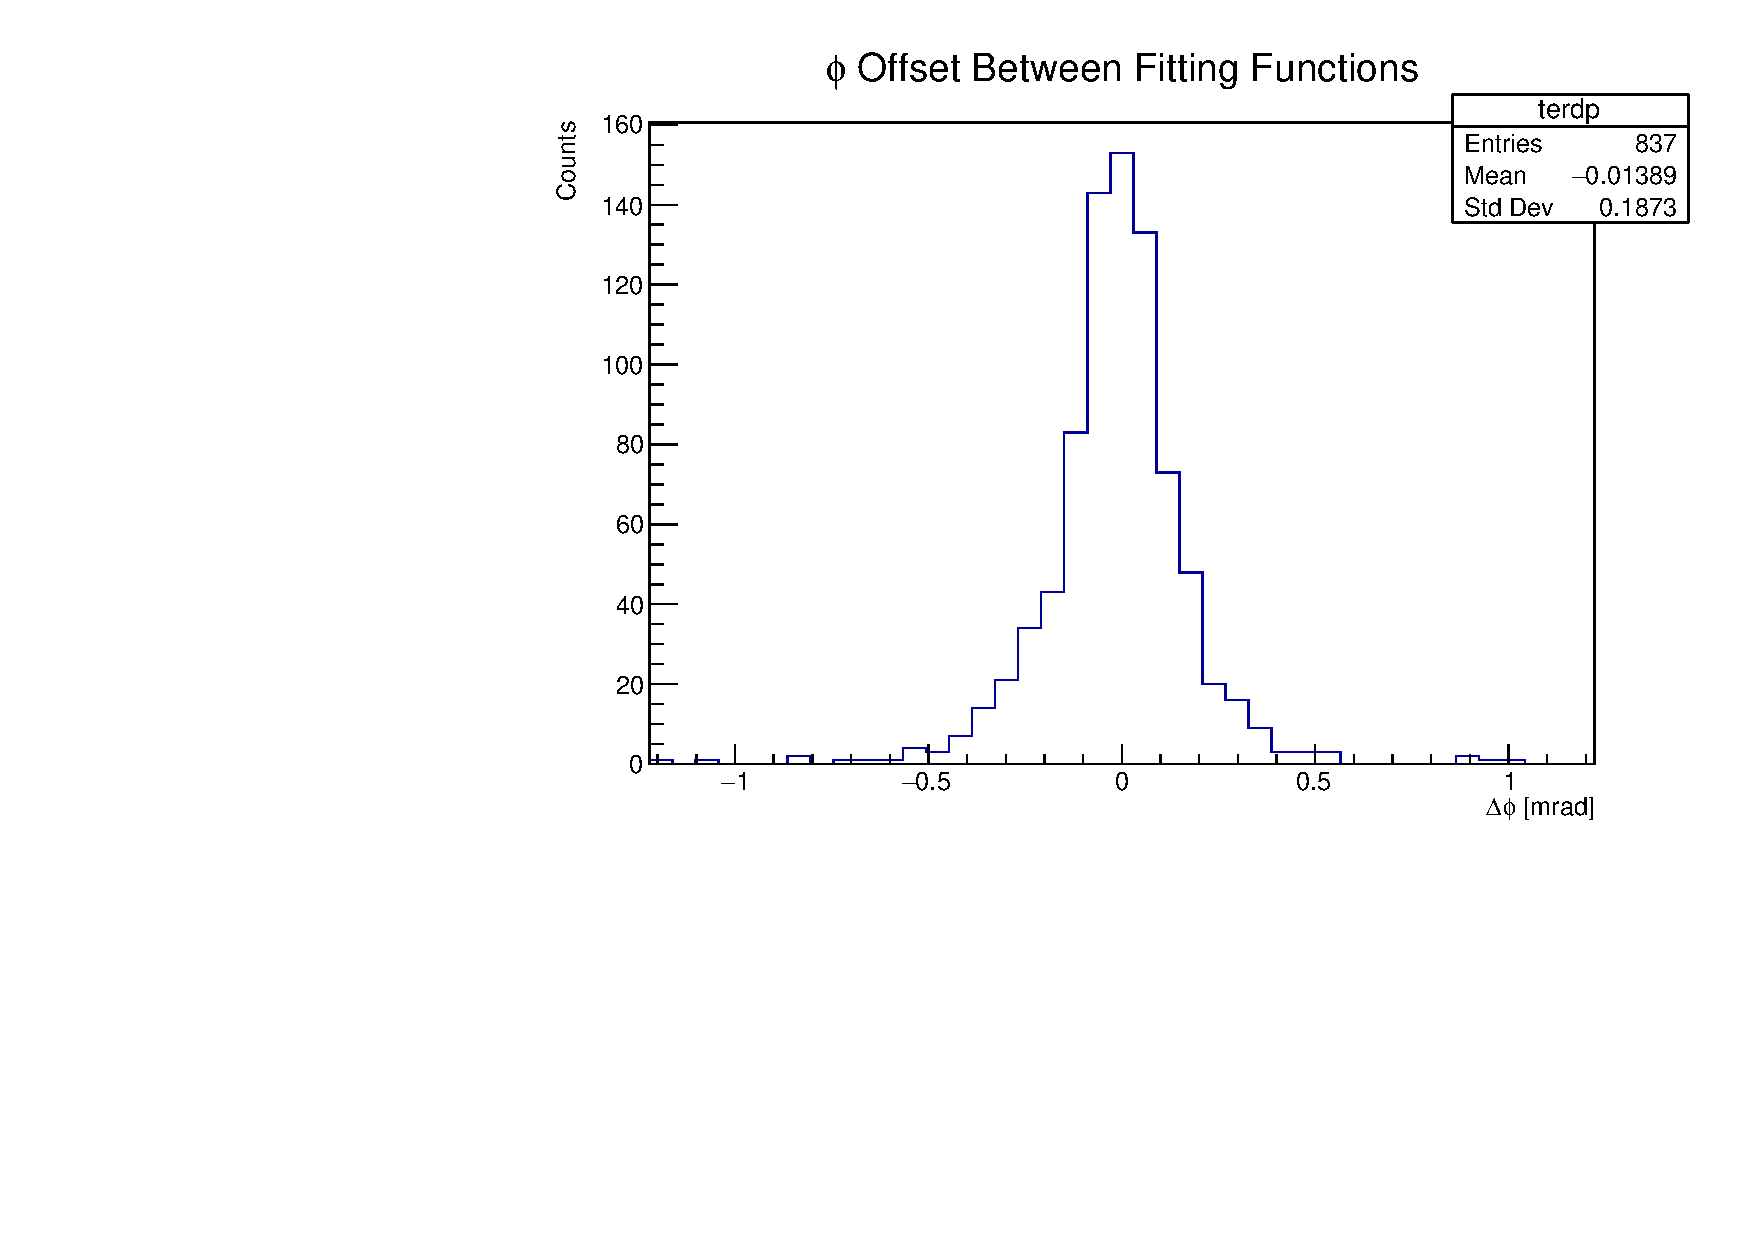
\includegraphics[width=.7\linewidth]{graphics/terdphc.pdf}
    \caption{Agreement In Found Z (top) and $\phi$ (bottom) Locations Between Fits}
    \label{fig:fitcompare}
\end{figure}

